\documentclass[a4paper]{article}
\usepackage{authblk}
%\usepackage{rotating}
%\usepackage{pdflscape}

\usepackage[bbgreekl]{mathbbol}
\usepackage{amssymb, amsmath, amsthm, stmaryrd}

\usepackage{array}
\usepackage{longtable}
\usepackage[usenames,dvipsnames]{color}   %colors
%\usepackage{colortbl}   %colorful tables
\usepackage{tabularx,tikz}
\usepackage{graphicx} %[dvips]
% it is note used \usepackage{cooltooltips}

%these two can be found in caption package
%\usepackage{caption}https://www.overleaf.com/project/5dbbf2c2d697d8000126aac9
%\usepackage{subcaption}

\usepackage[numbers]{natbib}
\usepackage{ulem}
\usepackage{etoolbox}
\usetikzlibrary{arrows,matrix}


%%%%%%%%%%%%%%%%%%%%%%%%%%%%%%%%%%%%%%%%%%%%%%%%%%%%%%%%%%%%%%%%%%%%%%%%%%%%
\newtheorem{theorem}{Theorem}
\newtheorem{corollary}[theorem]{Corollary}
\newtheorem{lemma}[theorem]{Lemma}

%%%%%%%%%%%%%%%%%%%% specific math macros
\def\abs#1{\lvert#1\rvert}
\def\Abs#1{\bigl\lvert#1\bigr\rvert}
\def\adiv{\widetilde\div}
\def\aep{\tilde\ep}
\def\agrad{\widetilde\nabla}
\def\avg#1{\left\{\mskip-5mu\left\{#1\right\}\mskip-5mu\right\}}
\def\CC{\tn C}
\def\d {\,{\rm d}}
\def\ddt#1{\frac{\d #1}{\d t}}
\def\dist{\operatorname{dist}}
\def\div{\operatorname{div}}
\def\dn{\d\nnu}
\def\dt{\prtl_t}
\def\dual#1#2{\left\langle #1,#2\right\rangle}
\def\ee{\vc e}
\def\ep{\vc\varepsilon}
\def\FF{\vc F}
\def\ff{\vc f}
\def\grad{\nabla}
% \def\Hel{\vc{\mathcal H}}
\def\Hf{\mathcal H}
\def\jmp#1{\left\llbracket #1 \right\rrbracket}
\def\Lapl{\Delta}
\def\Natural{\mathbf N}
\def\nn{\vc n}
\def\nnu{\vc\nu}
\def\norm#1{\left\|#1\right\|}
\def\ol{\overline}
\def\pbar{\overline p}
\def\pphi{{\varphi}}
\def\prtl{\partial}
\def\qq{\vc q}
\def\Real{{\mathbf R}}
\def\tn#1{{\mathbb{#1}}}    % tensor
\def\tr{\operatorname{tr}}
\def\tt{\vc t}
\def\U{\vc U}
\def\ubar{\overline\uu}
\def\ul{\underline}
\def\uu{\vc u}
\def\V{\vc V}
\def\Vel{{\vc{\mathcal V}}} % Sobolev space for elasticity
\def\Vf{{\mathcal V}} % Sobolev space for flow
\def\vc#1{\mathbf{\boldsymbol{#1}}}     % vector
\def\vv{\vc v}
\def\weakly{\rightharpoonup}
\def\xx{\vc x}
\def\yy{{\vc y}}
\def\O{\mathcal{O}}

\newcommand{\eq}[1]{\begin{equation}#1\end{equation}}
\newcommand{\eqs}[1]{\begin{equation*}#1\end{equation*}}
\newcommand{\ml}[1]{\begin{multline}#1\end{multline}}
\newcommand{\mls}[1]{\begin{multline*}#1\end{multline*}}

\newcommand{\note}[2]{{\color{blue} \textbf{ #1:} \textit{#2}}}
%% ini_table members
%%%%%%%%%%%%%%%%%%%% specific math macros

\newcommand{\opm}{ % plus and minus in circle
  {\mathbin{
    \mathchoice
      {\buildcirclepm{\displaystyle     }{0.14ex}{0.95}{0.05ex}{.7}}
      {\buildcirclepm{\textstyle        }{0.14ex}{0.95}{0.05ex}{.7}}
      {\buildcirclepm{\scriptstyle      }{0.13ex}{0.955}{0.04ex}{.55}}
      {\buildcirclepm{\scriptscriptstyle}{0.08ex}{0.95}{0.03ex}{.45}}
  }} 
}
\newcommand\buildcirclepm[5]{%
  \begin{tikzpicture}[baseline=(X.base), inner sep=-#5, outer sep=-.65]
    \node[draw,circle,line width=#4] (X)  {\footnotesize\raisebox{#2}{\scalebox{#3}{$#1\pm$}}};
  \end{tikzpicture}%
}


%%%%%%%%%%%%%%%%%%%%%%%%%%%%%%%%%%%%%%%%%%%%%%%%%%%%%%%%%%%%%%%%%%%%%%%%%%%%%%%%%%%%%%%%%%%%% BEGIN DOCUMENT
\begin{document}

\title{Mixed-dimensional models of linear elasticity and poroelasticity}
\author{Jan Březina}
\author{Jan Stebel}
\affil{Technical University of Liberec,\\ Studentská 1402/2, 461 17 Liberec, Czech Republic}
\affil{e-mail: \texttt{\{jan.brezina,jan.stebel\}@tul.cz}}
\maketitle


\section{Biot's system}

In this paper we describe a dimension reduction for the Biot system of poroelasticity in a domain containing a fracture, which is assumed to be a thin manifold around a subset of hyperplane.
The obtained equations (eq. \eqref{eq:lin_el_frac}, \eqref{eq:flow_frac}) are expressed in terms of mean pressure and mean displacement in the fracture.
The resulting problem consists of equations of flow and mechanics in the fracture and in the surrounding domain, accompanied by appropriate interface conditions (eq. \eqref{eq:interface_el}, \eqref{eq:interface_flow}).
Finally we analyse the well-posedness of the steady-state mechanical part of the problem.

The original idea of dimension reduction comes from \cite{martin_modeling_2005}, where it was applied to the darcian flow model.
Here we also deal with the linear elasticity system, for which the approach has to be generalized using tangential and normal calculus in the fracture.

The structure of the paper is as follows.
In section \ref{sec:model} we describe the original mathematical model and the full and reduced geometry.
The tangential and normal calculus is presented in section \ref{sec:calculus}.
In sections \ref{sec:reduction_elasticity} and \ref{sec:reduction_flow} we derive the reduced problem for mechanics and flow, respectively.
Finally, in section \ref{sec:wellposedness_elasticity} we prove the existence and uniqueness of weak solution to the mechanical part of the resulting problem.


\section{Biot's poroelasticity in domain with fracture}\label{sec:model}

\begin{figure}[h]
\centering
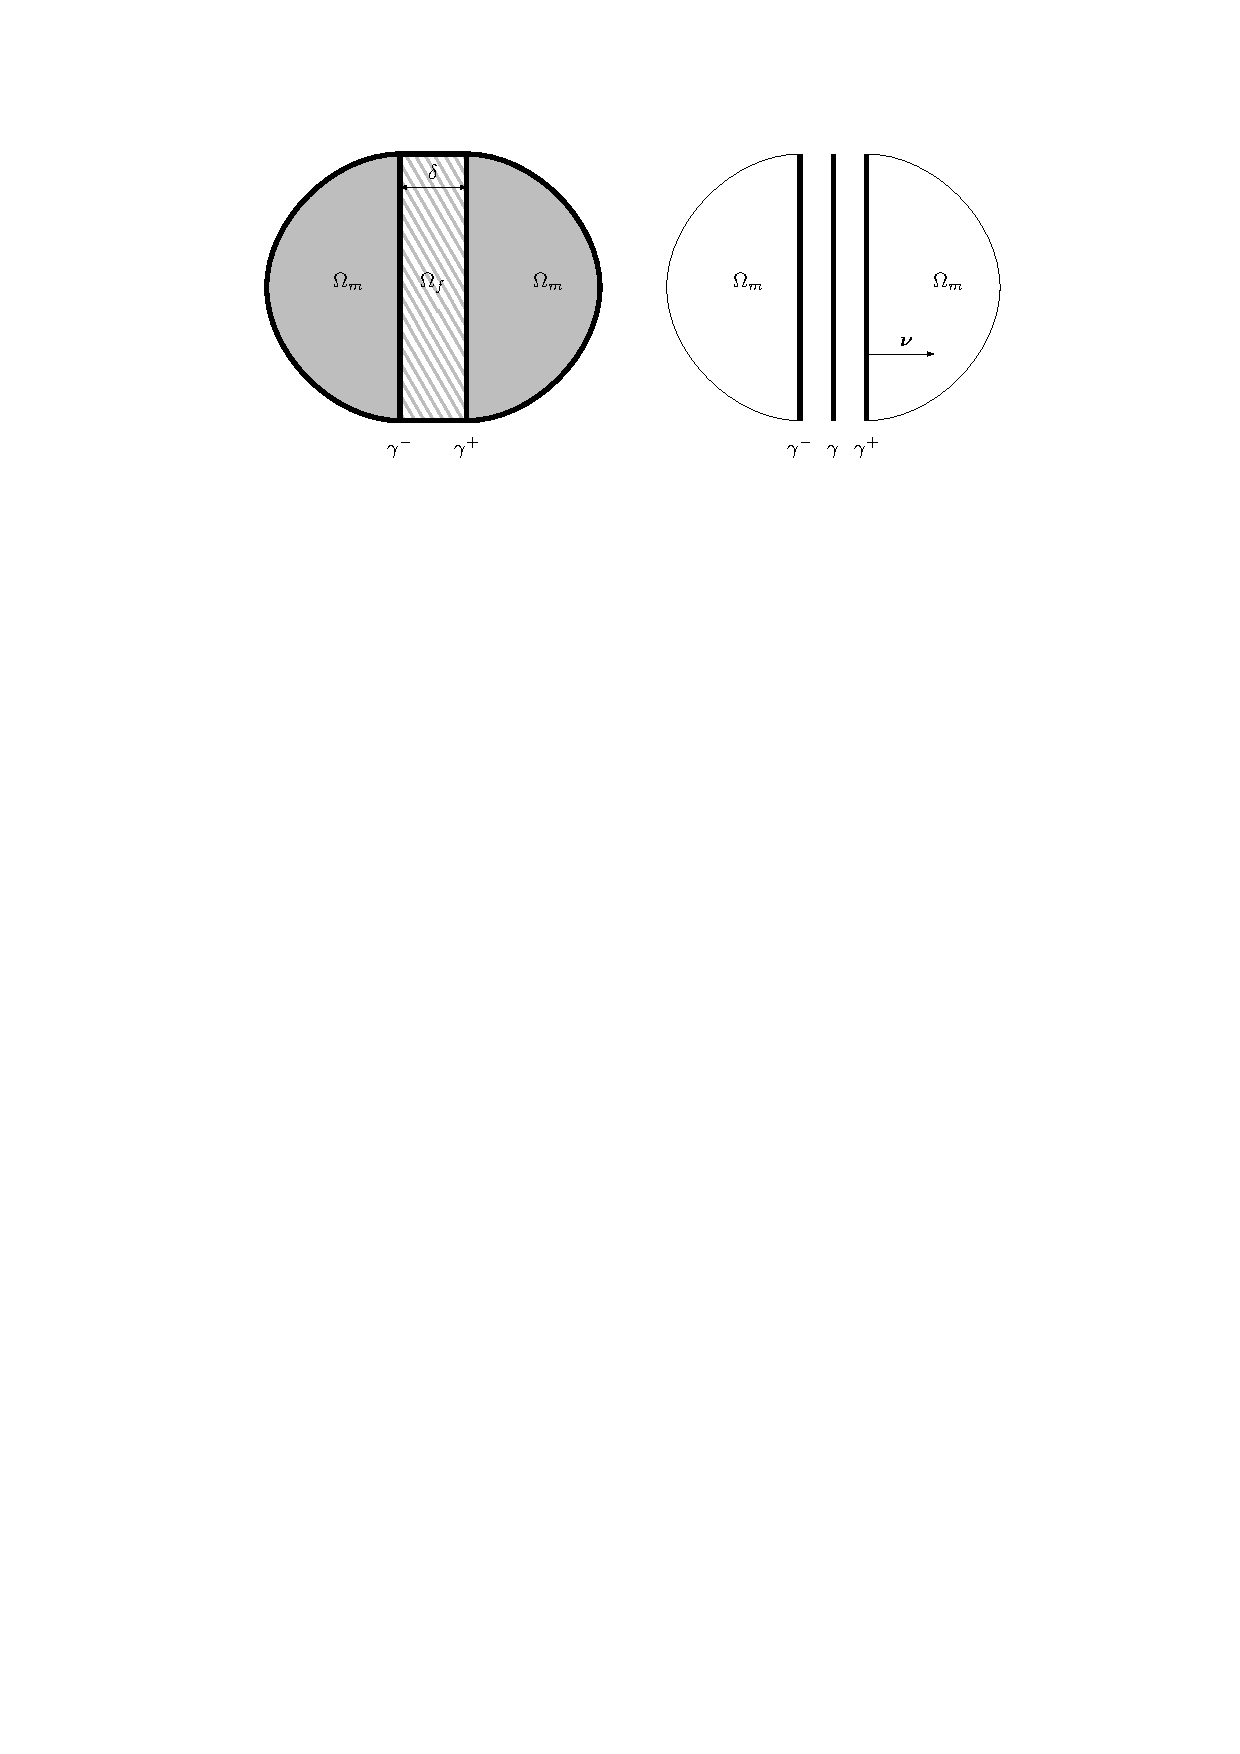
\includegraphics[width=\textwidth]{figures/omegas}
\caption{The domain of the full model (left) and the reduced geometry (right).}
\label{fig:omegas}
\end{figure}

Let $\Omega$ be a bounded, simply connected domain in the Euclidean space $\Real^d$, $d\in\{2,3\}$, with Lipschitz boundary $\partial\Omega$.
We assume that $\Omega$ is composed of two subdomains: the fracture $\Omega_f$ and the matrix $\Omega_m:=\Omega\setminus\overline\Omega_f$, and that the fracture divides the matrix into two parts (see Figure \ref{fig:omegas}).
For simplicity we consider straight fracture, i.e. there is a subset $\gamma$ of a hyperplane in $\Real^d$ and a number $\delta>0$ such that
\eqs{ \Omega_f = \{\xx+s\nnu;~\xx\in\gamma,~s\in(-\tfrac\delta2,\tfrac\delta2)\}, }
where $\nnu$ stands for the unit normal vector to $\gamma$.
The parameter $\delta$ is usually called the aperture or the width of the fracture.
% Choosing a suitable coordinate system we can take $\gamma:=\Omega\cap\left(\{0\}\times\Real^{d-1}\right)$ and $\nnu:=(1,0,0)^\top$ without loss of generality.
Then the two parts of $\Omega_m$ are interacting with $\Omega_f$ via the interfaces
\eqs{ \gamma^+ := \{\xx+\tfrac\delta2;~\xx\in\gamma\},\quad \gamma^- := \{\xx-\tfrac\delta2;~\xx\in\gamma\}. }
% \eq{ \gamma^+:=\Omega\cap\big( \{\tfrac\delta2\}\times \Real^{d-1}\big), \quad \gamma^-:=\Omega\cap\big( \{ -\tfrac\delta2\}\times \Real^{d-1}\big). }
The symbol $\prtl\gamma$ shall denote the relative boundary of $\gamma$.

% We shall derive a model of poroelasticity on the reduced geometry consisting of $\Omega_m$ and $\gamma$.
The basic hydro-mechanical interaction in a porous media is described by the Biot system of poroelasticity.
In context of this paper it reads:
\begin{subequations}
\label{eq:biot}
\begin{align}
    \label{eq:lin_el}
    -\div \bbsigma + \nabla(\alpha p) &= \ff &&\mbox{ in }\Omega_m\cup\Omega_f,\\
\label{eq:biot_darcy}    \dt\left(Sp + \div(\alpha\uu)\right) + \div\qq &= g &&\mbox{ in }\Omega_m\cup\Omega_f,
\end{align}
\end{subequations}
Here, the displacement $\uu$ and the pressure $p$ are the principal unknowns; further $\alpha$ is the Biot effective stress parameter, $\ff$ the body force, $S$ the storativity, $g$ the fluid source.
The stress tensor $\bbsigma$ is determined by the Hooke law:
\eqs{ \bbsigma = \CC\nabla\uu, }
where $\CC$ is the $4^{\rm th}$-order elasticity tensor.
The flux $\qq$ is given by the Darcy law:
\eqs{ \quad \qq = -\tn K\nabla p }
via the hydraulic conductivity tensor $\tn K$.
To complete the equations in $\Omega$, we require that
\eq{ \label{eq:continuity_on_gamma_pm} p,\uu,\qq\cdot\nnu,\bbsigma\nnu-\alpha p\nnu \mbox{ are continuous on } \gamma^\pm. }

In what follows, we shall assume that the physical parameters $\alpha,S,\CC,\tn K$ are constant in $\Omega_m$, $\Omega_f$, respectively.
To distinguish values in $\Omega_m$ and $\Omega_f$, we shall use the subscripts ``$m$'' and ``$f$'', i.e. $\alpha_m := \alpha_{|\Omega_m}$, $\alpha_f := \alpha_{|\Omega_f}$ etc.
In addition, it is assumed that $\CC_*$ and $\tn K_*$, $*\in\{m,f\}$, have the usual symmetries:
\eqs{ \forall \tn A,\tn B\in\Real^{d\times d}:~ \CC_*\tn A:\tn B=\CC_*\tn A^\top:\tn B=\CC_*\tn A:\tn B^\top=\CC_*\tn B:\tn A, }
\eqs{ \tn K_* = \tn K_*^\top, }
denoting by ``:'' the scalar product in $\Real^{d\times d}$, and possess the standard positive definiteness \cite{gurtin}:
There exist positive constants $\mu_m$, $\mu_f$, $\lambda_m$, $\lambda_f$, $\kappa_m$, $\kappa_f$, such that
\eq{ \label{eq:pos_def_C_gen} \forall\tn A\in\Real^{d\times d}:~\CC_*\tn A:\tn A \ge \mu_*\left|\tn A+\tn A^\top\right|^2 + \lambda_*|\tn I:\tn A|^2, }
\eq{ \label{eq:pos_def_K} \forall\vv\in\Real^d:~\tn K_*\vv\cdot\vv \ge \kappa_*|\vv|^2,\quad *\in\{m,f\}. }
Here
$|\tn A|$ denotes the Frobenius norm, i.e. $|\tn A|^2=\tn A:\tn A$.

\section{Reduction of elasticity eq}

matrix:
\eqs{
 -\div(\CC_m\nabla\uu) + \alpha_m\nabla p = \ff \qquad\mbox{ in }(0,T)\times\Omega_m,}
 

fracture:
\mls{
-\delta\div_{\tau} \CC^f_{\tau\tau} \nabla_{\tau} \U 
-\div_{\tau} \CC^f_{\tau\nu} \jmp{\nabla_{\nu}\uu}
-\jmp{C^f\nabla \uu}\nnu \\
+ \delta\alpha_f \nabla_\tau P 
+ \alpha_f\jmp{p}\nnu = \delta f
}



interface conditions:
\eqs{
\label{eq:mixed_dim_problem_int_el} (\CC_m(\nabla\uu)^\opm-\alpha_m p^\opm\tn I)\nnu = (\CC_f(\nabla\uu)^\opm-\alpha_f p^\opm\tn I)\nnu \qquad \mbox{ in }(0,T)\times\gamma,
}

weak:

\mls{
\int_{\Omega_m} \CC_m\nabla\uu : \nabla \vv 
-alpha_m p \div \vv\\
-\int_{\gamma} (\CC_m\nabla\uu^{\opm} 
- \alpha_m p^{\opm}\tn I)\nnu^{\opm} \cdot \vv^{\opm}
}


\end{document}


